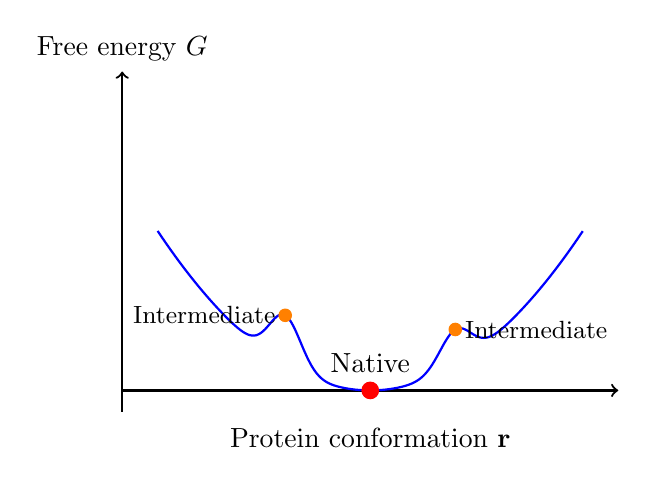
\begin{tikzpicture}[scale=1.5]
  % Define scaling factors
  \def\xscale{0.6}
  \def\yscale{0.6}
  
  % Function: f(x) = 0.25*x^2 + 0.7*exp(-10*(x+1.2)^2) + 0.5*exp(-10*(x-1.2)^2)
  % This creates a quadratic well with two local minima (intermediates)
  
  % Draw axes
  \draw[->, thick] (-3.5*\xscale,0) -- (3.5*\xscale,0) node[right] {};
  \draw[->, thick] (-3.5*\xscale,-0.3*\yscale) -- (-3.5*\xscale,4.5*\yscale) node[above] {Free energy $G$};
  
  % Plot the energy landscape
  \draw[thick, blue, smooth] plot[domain=-3:3, samples=100] 
    ({(\x)*\xscale}, {(0.25*\x*\x + 0.7*exp(-10*(\x+1.2)*(\x+1.2)) + 0.5*exp(-10*(\x-1.2)*(\x-1.2)))*\yscale});
  
  % Mark the native state (global minimum at x=0)
  \filldraw[red] (0,0) circle (2pt);
  \node[above=3pt] at (0,0) {Native};
  \node[below=10pt] at (0,0) {Protein conformation $\mathbf{r}$};
  
  % Mark intermediate states (local minima at x ≈ ±1.2)
  \filldraw[orange] ({-1.2*\xscale},{(0.25*1.44 + 0.7)*\yscale}) circle (1.5pt);
  \node[left, font=\small] at ({-1.2*\xscale},{(0.25*1.44 + 0.7)*\yscale}) {Intermediate};
  
  \filldraw[orange] ({1.2*\xscale},{(0.25*1.44 + 0.5)*\yscale}) circle (1.5pt);
  \node[right, font=\small] at ({1.2*\xscale},{(0.25*1.44 + 0.5)*\yscale}) {Intermediate};
  
\end{tikzpicture}